% Generado por informe-oficial/figuras/dominios.py (lo llama generar-figuras.sh) desde el ER de la base y la tabla «Dominios del modelo»
% de docs/08. No editar a mano: lo comprueba generar-figuras.sh --verificar.

\begin{figure}[!htbp]
\centering
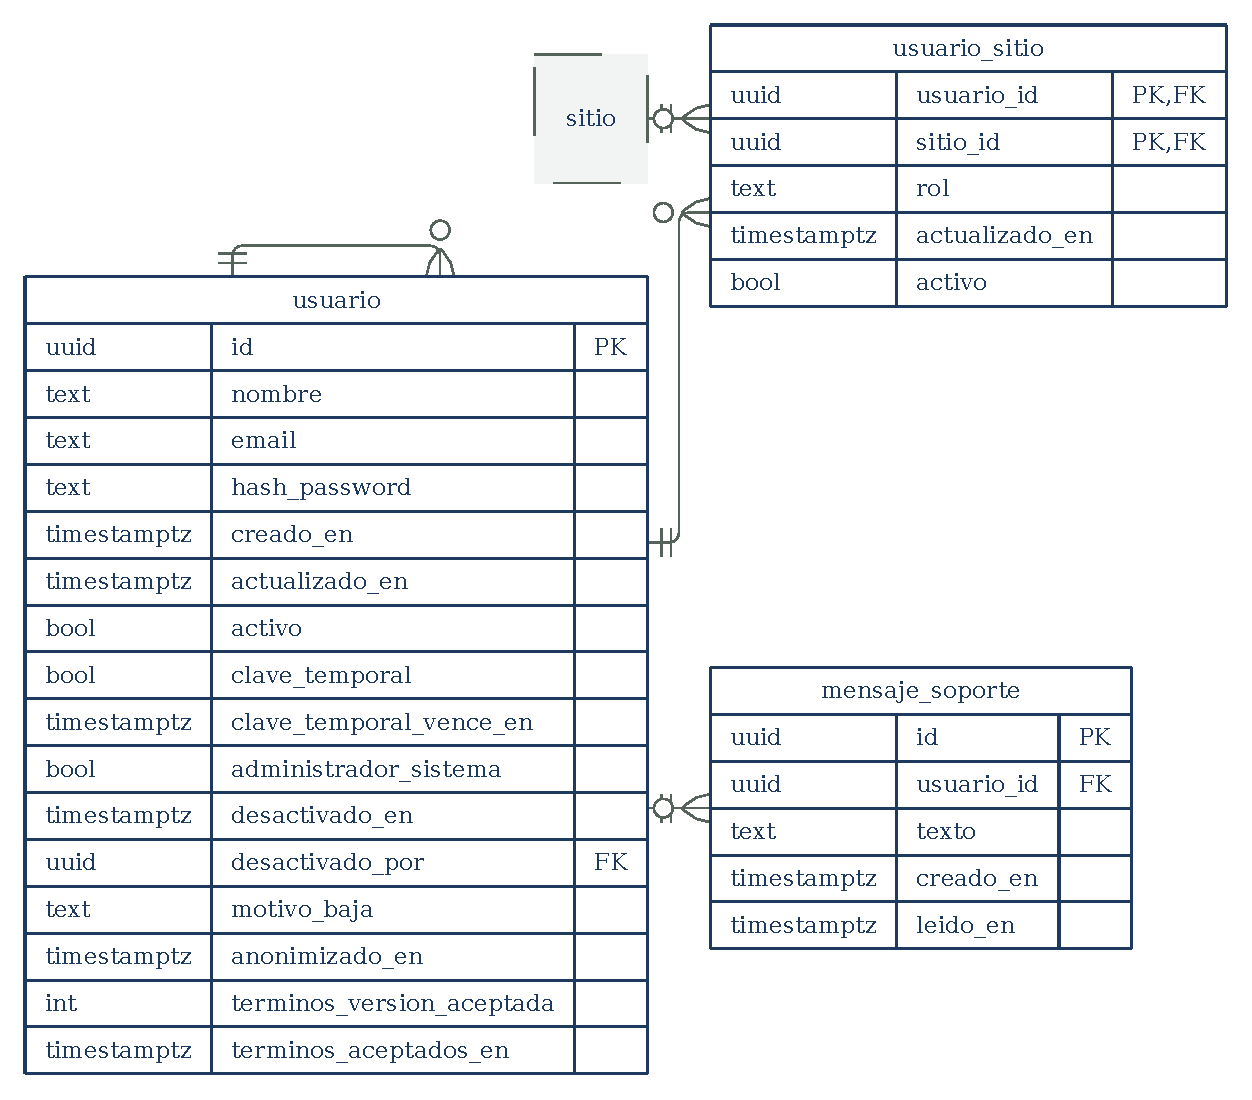
\includegraphics[width=\linewidth,height=0.82\textheight,keepaspectratio]{figuras/render/modelo-cuentas-y-sesion-1.pdf}
\caption[Modelo de datos: Cuentas y sesión (parte 1 de 2)]{Modelo de datos, dominio «Cuentas y sesión» (parte 1 de 2). Las personas: quién entra a qué sitio y con qué rol, sus sesiones e intentos de acceso, sus preferencias y sus mensajes de soporte. Tablas de esta figura: \texttt{usuario}, \texttt{usuario\_sitio}, \texttt{mensaje\_soporte}. Con borde punteado y sin columnas, las tablas a las que apuntan claves foráneas de estas y que se dibujan en otra figura: \texttt{sitio}.}
\label{fig:modelo-cuentas-y-sesion-1}
\end{figure}

\begin{figure}[!htbp]
\centering
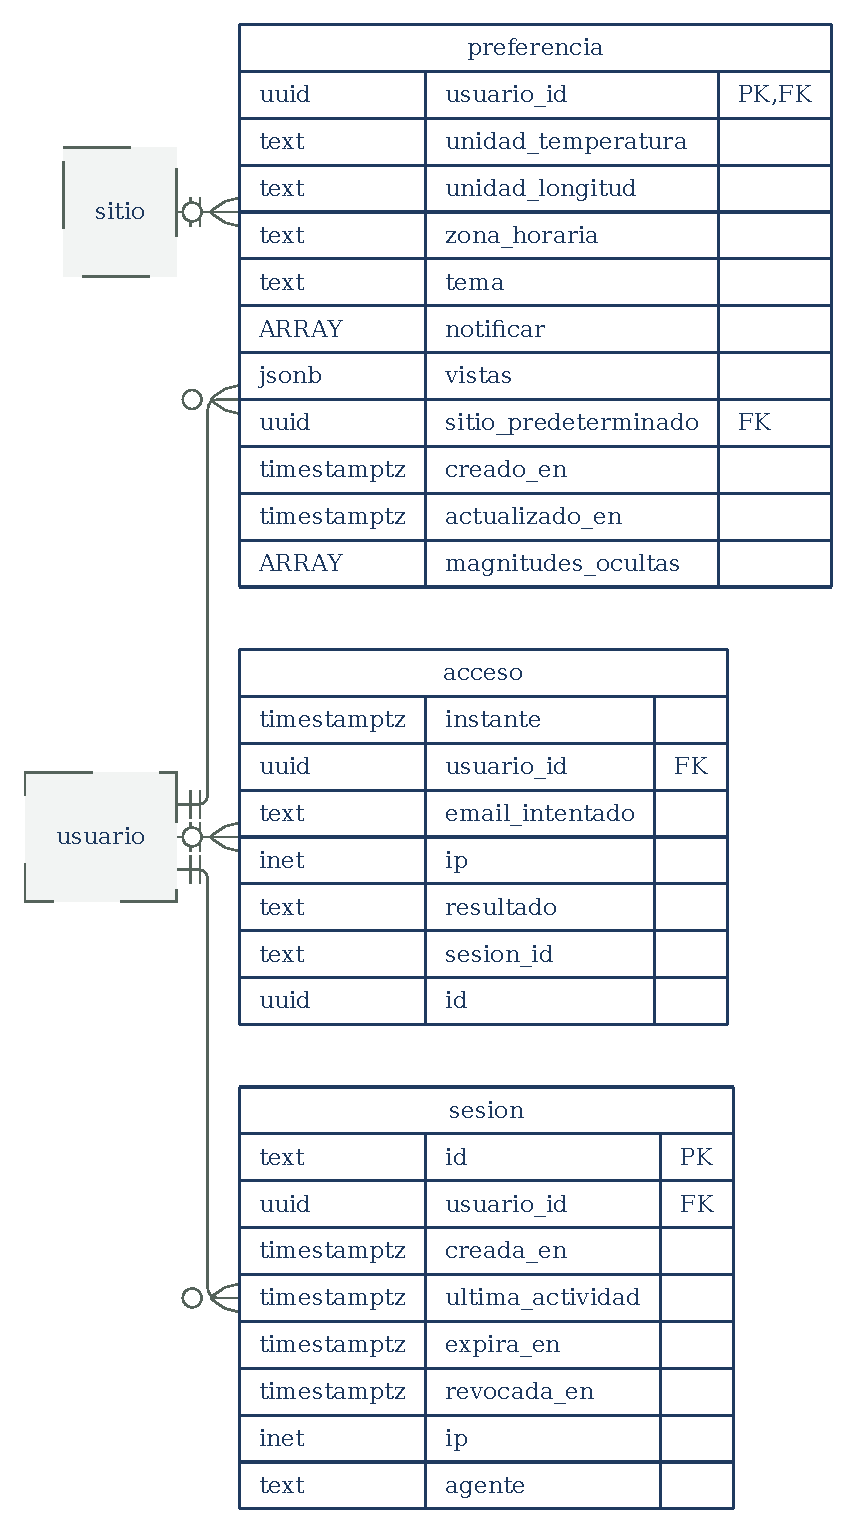
\includegraphics[width=\linewidth,height=0.82\textheight,keepaspectratio]{figuras/render/modelo-cuentas-y-sesion-2.pdf}
\caption[Modelo de datos: Cuentas y sesión (parte 2 de 2)]{Modelo de datos, dominio «Cuentas y sesión» (parte 2 de 2). Tablas de esta figura: \texttt{sesion}, \texttt{acceso}, \texttt{preferencia}. Con borde punteado y sin columnas, las tablas a las que apuntan claves foráneas de estas y que se dibujan en otra figura: \texttt{sitio}, \texttt{usuario}.}
\label{fig:modelo-cuentas-y-sesion-2}
\end{figure}

\begin{figure}[!htbp]
\centering
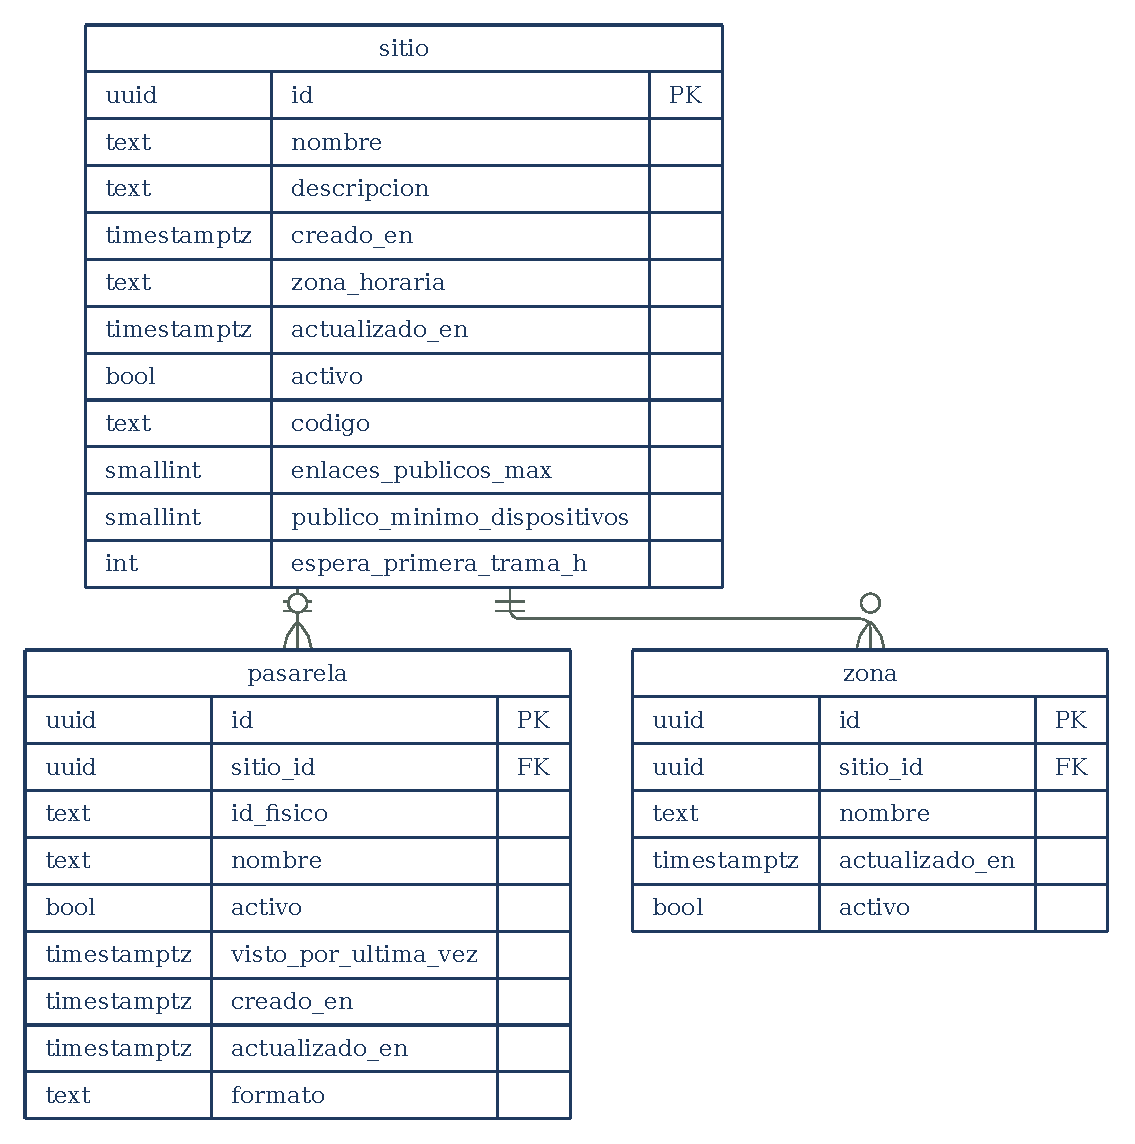
\includegraphics[width=\linewidth,height=0.82\textheight,keepaspectratio]{figuras/render/modelo-sitios-y-dispositivos-1.pdf}
\caption[Modelo de datos: Sitios y dispositivos (parte 1 de 4)]{Modelo de datos, dominio «Sitios y dispositivos» (parte 1 de 4). El inventario: dónde está cada equipo, quién lo identifica ante el broker, qué magnitudes reporta y cuál es su estado actual; y el catálogo con que se lee lo que envía (magnitudes, alias y recetas de decodificación). Tablas de esta figura: \texttt{sitio}, \texttt{zona}, \texttt{pasarela}.}
\label{fig:modelo-sitios-y-dispositivos-1}
\end{figure}

\begin{figure}[!htbp]
\centering
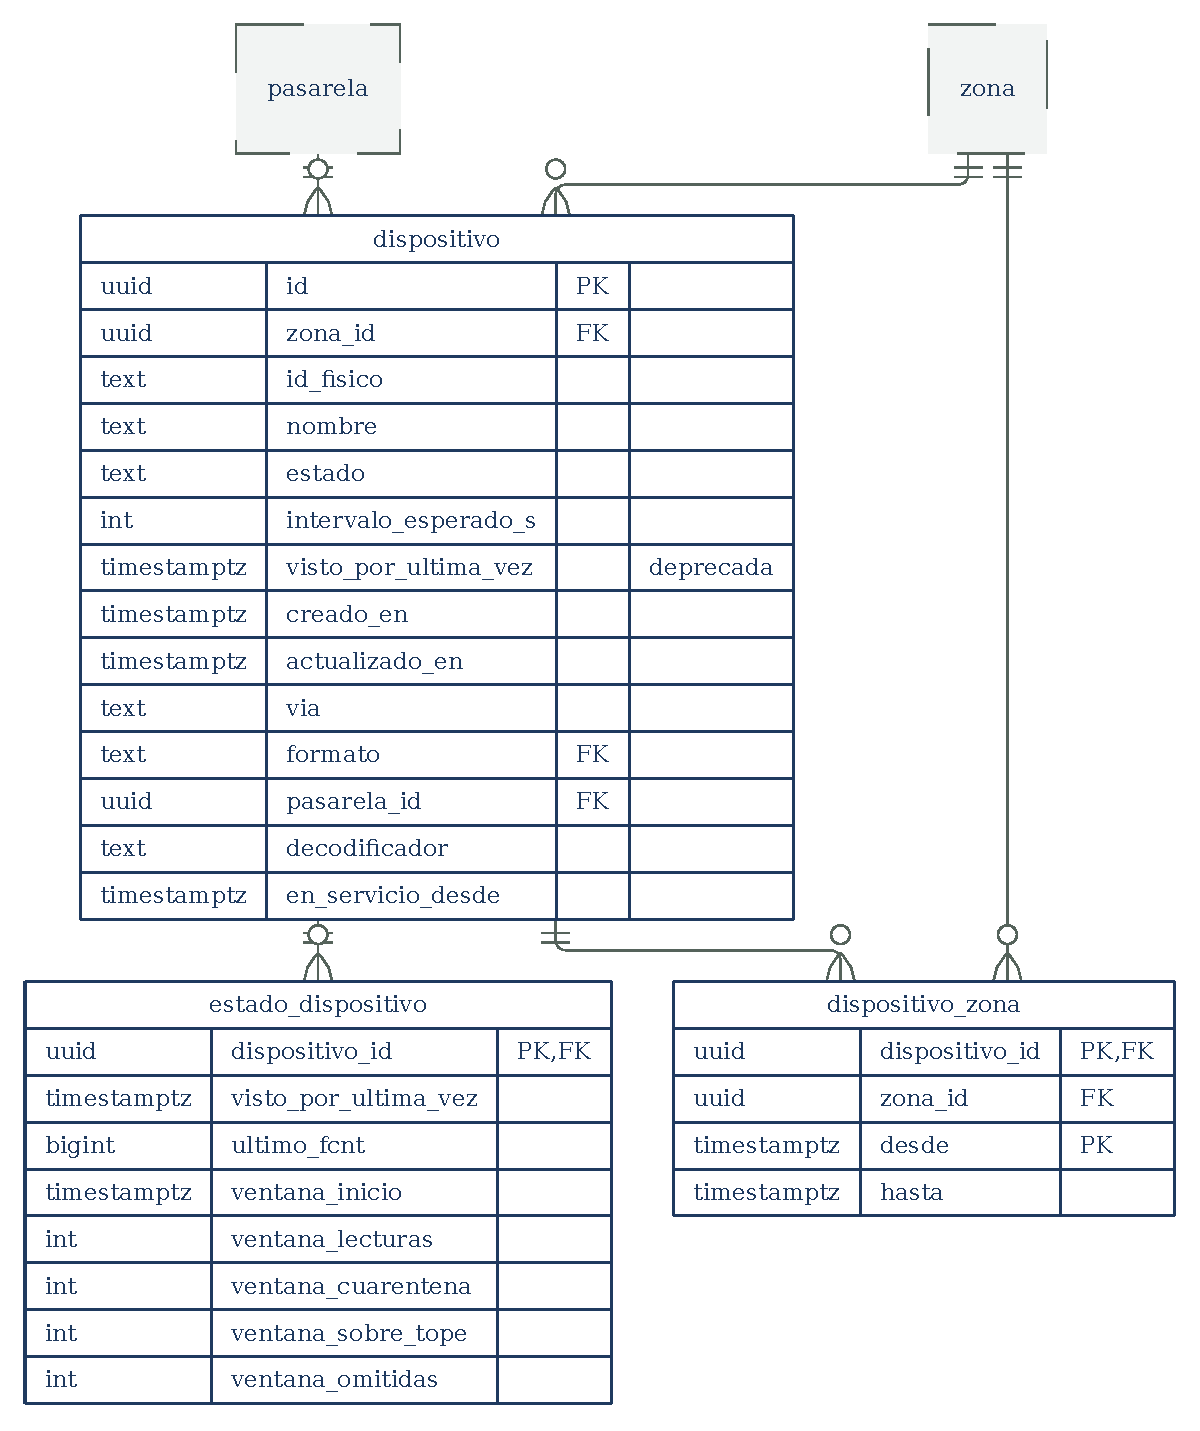
\includegraphics[width=\linewidth,height=0.82\textheight,keepaspectratio]{figuras/render/modelo-sitios-y-dispositivos-2.pdf}
\caption[Modelo de datos: Sitios y dispositivos (parte 2 de 4)]{Modelo de datos, dominio «Sitios y dispositivos» (parte 2 de 4). Tablas de esta figura: \texttt{dispositivo}, \texttt{dispositivo\_zona}, \texttt{estado\_dispositivo}. Con borde punteado y sin columnas, las tablas a las que apuntan claves foráneas de estas y que se dibujan en otra figura: \texttt{pasarela}, \texttt{receta\_decodificacion}, \texttt{zona}.}
\label{fig:modelo-sitios-y-dispositivos-2}
\end{figure}

\begin{figure}[!htbp]
\centering
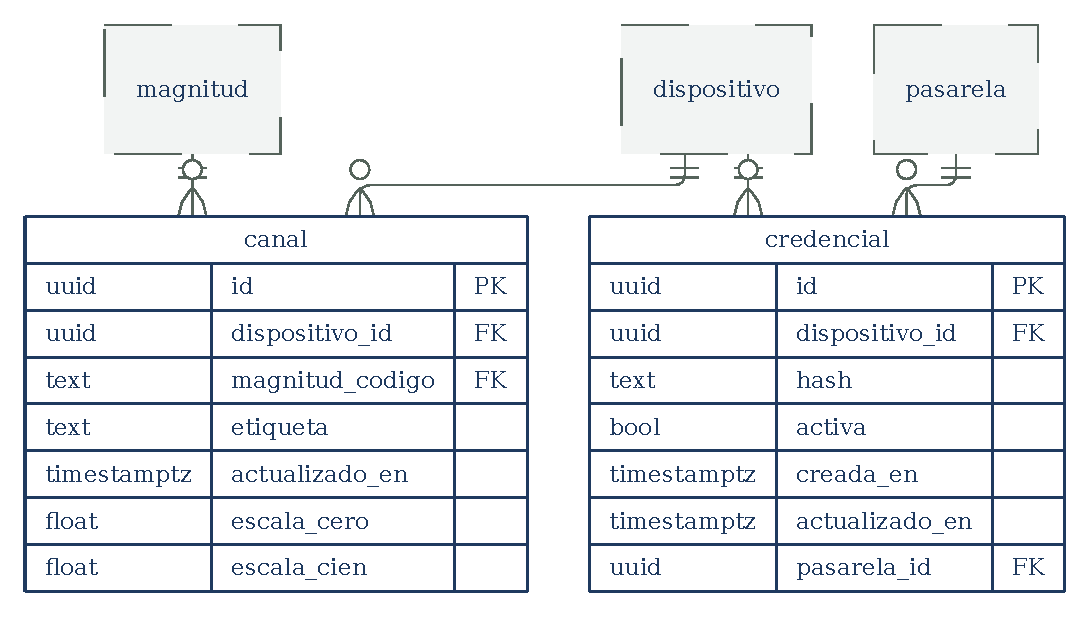
\includegraphics[width=\linewidth,height=0.82\textheight,keepaspectratio]{figuras/render/modelo-sitios-y-dispositivos-3.pdf}
\caption[Modelo de datos: Sitios y dispositivos (parte 3 de 4)]{Modelo de datos, dominio «Sitios y dispositivos» (parte 3 de 4). Tablas de esta figura: \texttt{credencial}, \texttt{canal}. Con borde punteado y sin columnas, las tablas a las que apuntan claves foráneas de estas y que se dibujan en otra figura: \texttt{dispositivo}, \texttt{magnitud}, \texttt{pasarela}.}
\label{fig:modelo-sitios-y-dispositivos-3}
\end{figure}

\begin{figure}[!htbp]
\centering
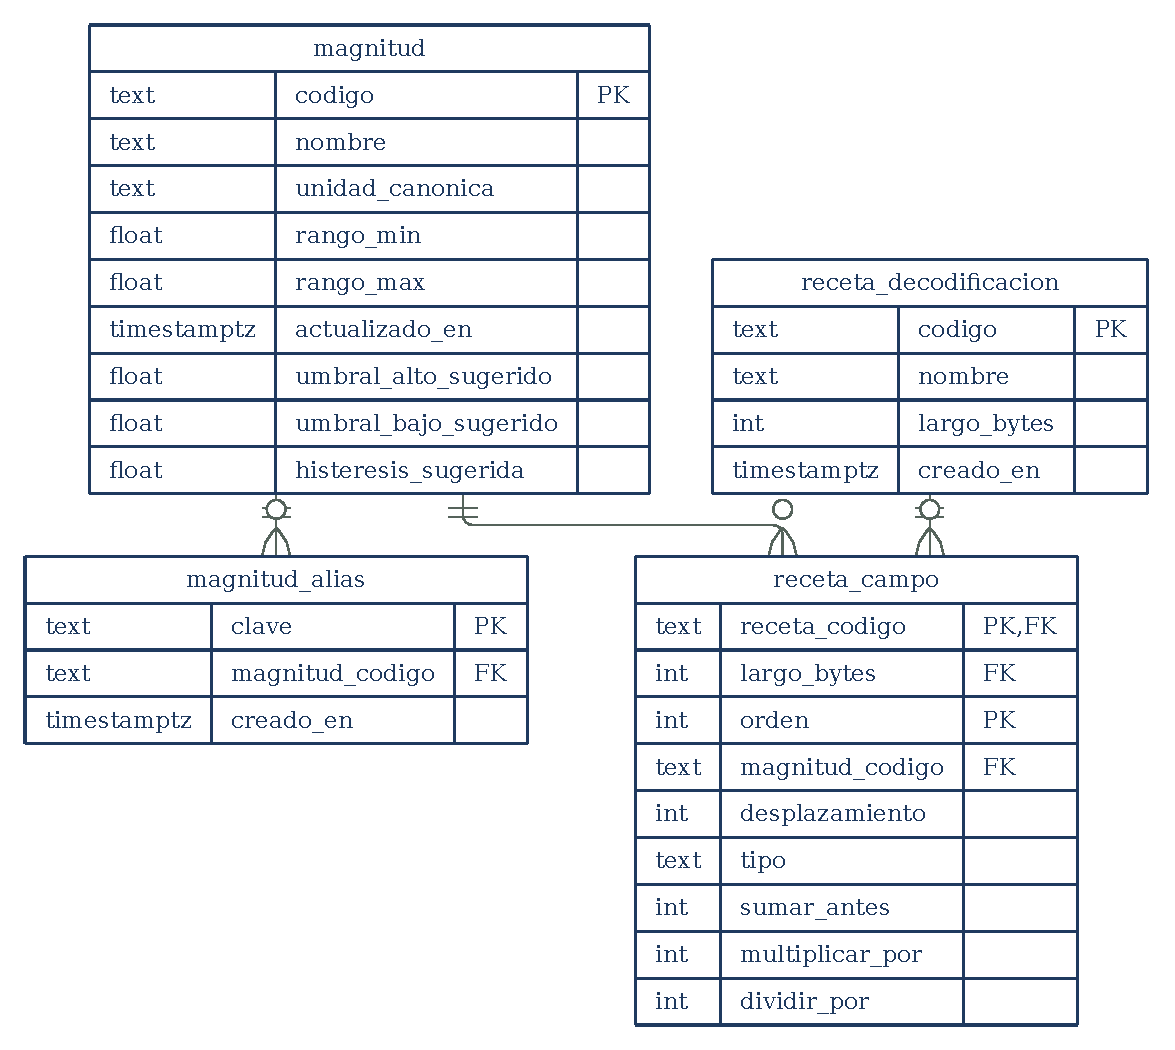
\includegraphics[width=\linewidth,height=0.82\textheight,keepaspectratio]{figuras/render/modelo-sitios-y-dispositivos-4.pdf}
\caption[Modelo de datos: Sitios y dispositivos (parte 4 de 4)]{Modelo de datos, dominio «Sitios y dispositivos» (parte 4 de 4). Tablas de esta figura: \texttt{magnitud}, \texttt{magnitud\_alias}, \texttt{receta\_decodificacion}, \texttt{receta\_campo}.}
\label{fig:modelo-sitios-y-dispositivos-4}
\end{figure}

\begin{figure}[!htbp]
\centering
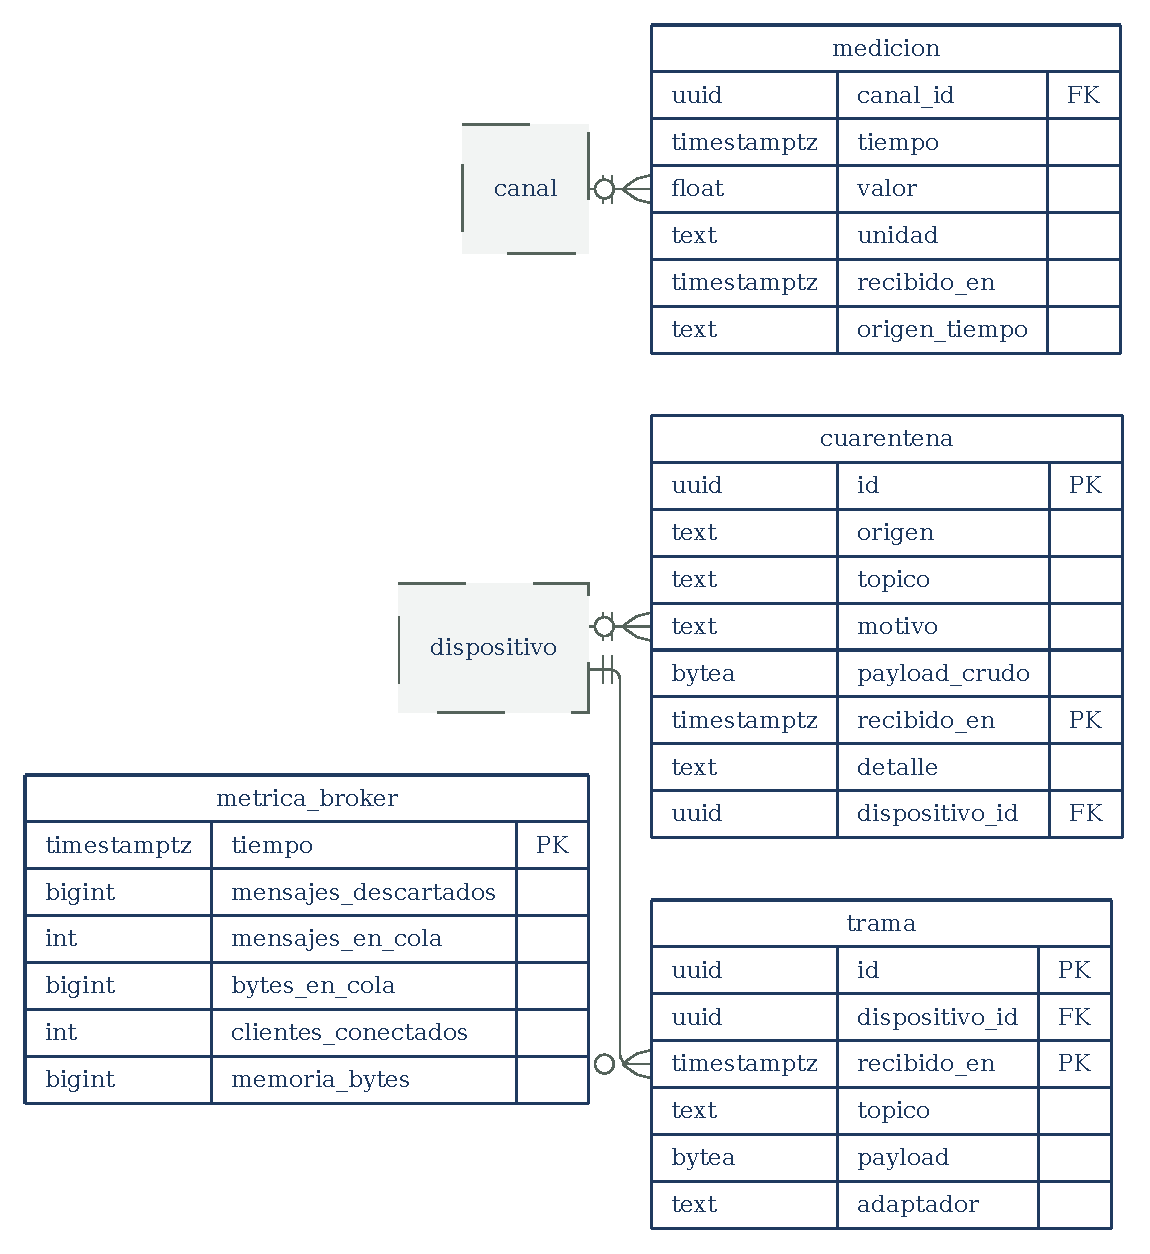
\includegraphics[width=\linewidth,height=0.82\textheight,keepaspectratio]{figuras/render/modelo-recepcion-y-mediciones.pdf}
\caption[Modelo de datos: Recepción y mediciones]{Modelo de datos, dominio «Recepción y mediciones». Lo que entra: la trama cruda aceptada o rechazada, la serie de tiempo normalizada y las muestras del propio broker. Tablas de esta figura: \texttt{trama}, \texttt{cuarentena}, \texttt{medicion}, \texttt{metrica\_broker}. Con borde punteado y sin columnas, las tablas a las que apuntan claves foráneas de estas y que se dibujan en otra figura: \texttt{canal}, \texttt{dispositivo}.}
\label{fig:modelo-recepcion-y-mediciones}
\end{figure}

\begin{figure}[!htbp]
\centering
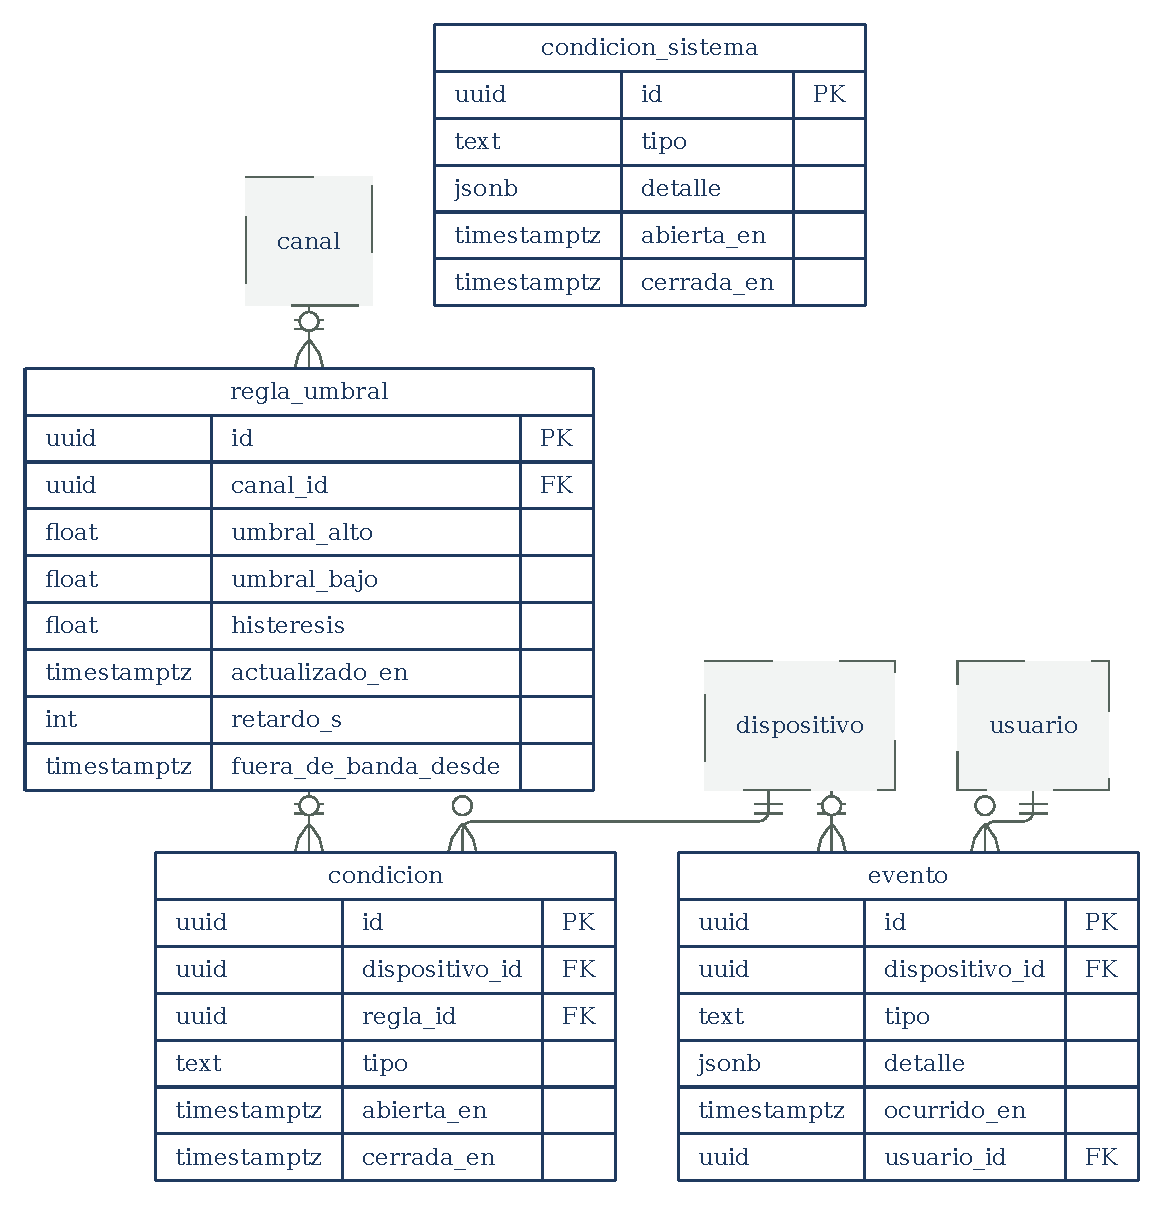
\includegraphics[width=\linewidth,height=0.82\textheight,keepaspectratio]{figuras/render/modelo-alertas-y-actividad.pdf}
\caption[Modelo de datos: Alertas y actividad]{Modelo de datos, dominio «Alertas y actividad». Lo que el sistema vigila y lo que pasó: umbrales, estados anómalos abiertos y el registro histórico. Tablas de esta figura: \texttt{regla\_umbral}, \texttt{condicion}, \texttt{condicion\_sistema}, \texttt{evento}. Con borde punteado y sin columnas, las tablas a las que apuntan claves foráneas de estas y que se dibujan en otra figura: \texttt{canal}, \texttt{dispositivo}, \texttt{usuario}.}
\label{fig:modelo-alertas-y-actividad}
\end{figure}

\begin{figure}[!htbp]
\centering
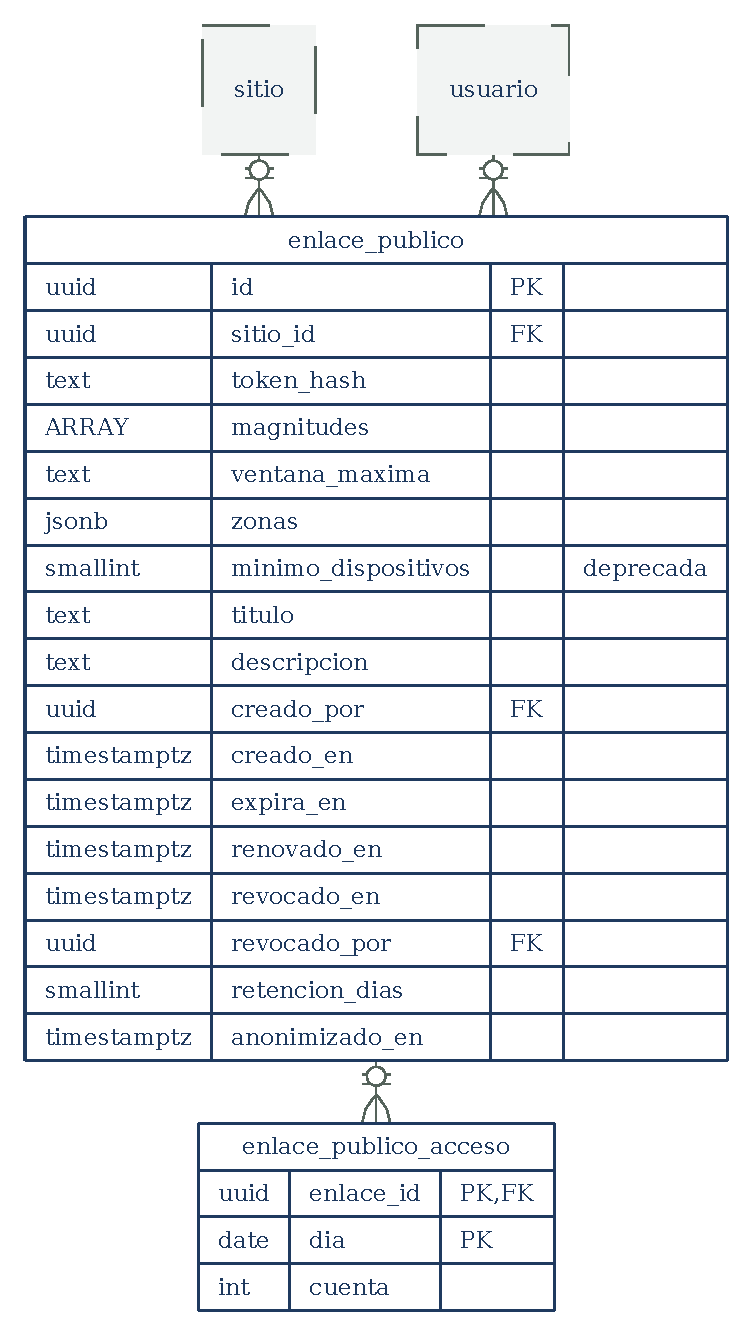
\includegraphics[width=\linewidth,height=0.82\textheight,keepaspectratio]{figuras/render/modelo-vista-publica.pdf}
\caption[Modelo de datos: Vista pública]{Modelo de datos, dominio «Vista pública». Los enlaces que publican una vista de un sitio sin iniciar sesión, y su contador de visitas. Tablas de esta figura: \texttt{enlace\_publico}, \texttt{enlace\_publico\_acceso}. Con borde punteado y sin columnas, las tablas a las que apuntan claves foráneas de estas y que se dibujan en otra figura: \texttt{sitio}, \texttt{usuario}.}
\label{fig:modelo-vista-publica}
\end{figure}
